\documentclass[11pt,aps,preprint,nofootinbib,superscriptaddress,tightenlines]{revtex4-2}
\usepackage{amsmath,amssymb,bm,mathtools}
\usepackage{graphicx}
\usepackage{xcolor}
\definecolor{darkblue}{RGB}{0,0,160}
\usepackage[colorlinks=true,linkcolor=darkblue,citecolor=darkblue,urlcolor=darkblue]{hyperref}

\def\st{\begin{equation}}
\def\stp{\end{equation}}
\def\Eq#1{eq.~(\ref{#1})}
\def\Sect#1{Sect.~\ref{#1}}
\def\Fig#1{Fig.~\ref{#1}}
\usepackage{dsfont}
\newcommand{\one}{\mathds{1}}
\let\oldparagraph\paragraph
\renewcommand{\paragraph}{\par\bigskip\oldparagraph}

\begin{document}

\title{Changing the particle representation for the viscous step}
\author{D.~Teaney}
\affiliation{Department of Physics and Astronomy, Stony Brook University,
Stony Brook, New York 11794, USA}
\date{\today}

\begin{abstract}
The Hamiltonian step works with smoothed fields, and the thermodynamic force it
provides, $\beta_a$, is the fluid velocity smoothed twice.  Any viscous step
built on $\beta_a$ damps short wavelengths at most as fast as the smoothing
lets through, a factor $R(k)^2$.  Here the viscous step is done instead in a
particle representation.  Each particle is given its own energy $e_a$, which is
held fixed during the viscous step.  Momentum is transferred between particles
so that the total particle entropy $\sum_aS_a(e_a,\bm m_a)$ increases, and the
thermodynamic force is the particle's own $\beta_a=-\partial S_a/\partial\bm m_a$.
After the step the particles have the same energies, new momenta and new
entropies, and the next Hamiltonian step proceeds from there.  We relate the
particle energies to the smoothed energy $H$ to quadratic order, and test the
deterministic version: on a lattice the damping rate changes from
$\Gamma_{\rm phys}R^2B$ to $\Gamma_{\rm phys}B$, in 1D and 2D.
\end{abstract}

\maketitle

%=============================================================================
\section{Two representations}
\label{sec:reps}

Each particle carries an entropy $s_a$ and a momentum $\bm m_a$, and sits at
$\bm x_a$.  The positions do not change during the viscous step.

\paragraph{The smoothed representation.}  The Hamiltonian step uses the
smoothed densities at the particle,
\st
S_a=\sum_bs_b\,W_{ab},\qquad \bm M_a=\sum_b\bm m_b\,W_{ab},
\stp
and the energy
\st
H=\sum_aH_a,\qquad H_a=s_a\,\mathcal E(S_a,\bm M_a),
\label{H}
\stp
where $\mathcal E(S,\bm M)$ is the energy per unit entropy of a fluid with
entropy density $S$ and momentum density $\bm M$.  Its thermodynamic force is
\st
\beta_a=\frac{\partial H/\partial\bm m_a}{\partial H/\partial s_a}
=\frac{\dot{\bm x}_a}{\partial H/\partial s_a} .
\stp
It contains two smoothings: one to form $\bm M$, and one in
$\partial H/\partial\bm m_a=\dot{\bm x}_a=\sum_bV_b\,\bm v_bW_{ab}$, because
varying $\bm m_a$ changes $\bm M$ at every neighbour.

\paragraph{The particle representation.}  Give each particle the volume
\st
V_a=\frac{s_a}{S_a},
\stp
so that its own entropy density is the smoothed one.  Its own momentum density
is $\bm m_a/V_a$.  The equation of state then assigns it an energy and,
inversely, an entropy:
\st
e_a=E_a(s_a,\bm m_a)\equiv V_a\,h\Big(\frac{s_a}{V_a},\frac{\bm m_a}{V_a}\Big),\qquad
s_a=S_a(e_a,\bm m_a)\equiv V_a\,\sigma\Big(\frac{e_a}{V_a},\frac{\bm m_a}{V_a}\Big).
\label{Ea}
\stp
Here $h=S\mathcal E$ is the energy density as a function of the entropy and
momentum densities, and $\sigma$ the entropy density as a function of the energy
and momentum densities.  The two relations are inverse to each other at fixed
$V_a$.  The volume is a property of the particle, not a third variable: it is
fixed by the configuration and held fixed during the viscous step.

\paragraph{Derivatives.}  From the thermodynamic identity
$de=T\,ds+\bm v\cdot d\bm m$ at fixed $V_a$,
\st
\frac{\partial S_a}{\partial e_a}=\frac1{T_a},\qquad
\frac{\partial S_a}{\partial\bm m_a}=-\frac{\bm v_a}{T_a}\equiv-\beta_a ,
\label{betapt}
\stp
where $\bm v_a$ and $T_a$ are the velocity and temperature at the particle's
own densities.  ($T_a=(e+p)/S$ is the code's density-frame temperature,
$T_{\rm rel}/\gamma$.)  So $\beta_a$ is the particle's own thermodynamic force.
At rest, to linear order, $\beta_a=\bm m_a/(V_a\,wT)$: proportional to the
particle's own momentum, with no smoothing.

%=============================================================================
\section{Particle energies and the smoothed energy}
\label{sec:energies}

The particle energies \Eq{Ea} and the smoothed energies \Eq{H} differ only in
the momentum argument.  Write the momentum per unit entropy of a particle and
its smoothed average as
\st
\bm\mu_a=\frac{\bm m_a}{s_a},\qquad
\bar{\bm\mu}_a=\frac{\bm M_a}{S_a}=\sum_b\lambda_{ab}\,\bm\mu_b,\qquad
\lambda_{ab}=\frac{s_bW_{ab}}{S_a},\quad\sum_b\lambda_{ab}=1 .
\stp
Then
\st
e_a=s_a\,f_a(\bm\mu_a),\qquad H_a=s_a\,f_a(\bar{\bm\mu}_a),\qquad
f_a(\bm\mu)\equiv\mathcal E(S_a,S_a\bm\mu) .
\stp
The function $f_a$ is the energy per unit entropy at the density $S_a$, as a
function of the momentum per unit entropy.  Its derivatives are the velocity
and the inverse susceptibility,
\st
\frac{\partial f_a}{\partial\bm\mu}=\bm v,\qquad
\frac{\partial^2f_a}{\partial\bm\mu\,\partial\bm\mu}=C_a ,
\stp
with $C_a$ positive definite ($C_a=\one/T$ at rest).

\paragraph{Convexity.}  Since $f_a$ is convex, Jensen's inequality gives
$f_a(\bar{\bm\mu}_a)\le\sum_b\lambda_{ab}f_a(\bm\mu_b)$.  Summing over $a$ with
weight $s_a$, and using that $\sum_as_aW_{ab}/S_a\simeq1$ and that $S_a$ varies
slowly across a star,
\st
H\le\sum_ae_a .
\stp
The particle energies exceed the smoothed energy by the energy of the momentum
fluctuations that the smoothing averages away.  This is the energy form of the
entropy inequality $S(\underline P)\ge\underline S$ of \texttt{sph1.tex}.

\paragraph{Quadratic order.}  Expand the smoothed energy at particle $a$, not
the particle's own energy.  For each neighbour $b$ write
$\delta\bm\mu_{ab}=\bm\mu_b-\bar{\bm\mu}_a$, the deviation of its momentum per
unit entropy from the local average at $a$.  Then
\st
\sum_b\lambda_{ab}\,f_a(\bm\mu_b)
=f_a(\bar{\bm\mu}_a)+\bar{\bm v}_a\cdot\sum_b\lambda_{ab}\,\delta\bm\mu_{ab}
+\frac12\sum_b\lambda_{ab}\,\delta\bm\mu_{ab}\cdot C_a\cdot\delta\bm\mu_{ab}+\dots
\stp
The linear term vanishes identically, because the average is taken with the
same weights that define it:
\st
\sum_b\lambda_{ab}\,\delta\bm\mu_{ab}=0 .
\stp
Multiply by $s_a$ and sum over $a$.  On the left,
\st
\sum_as_a\sum_b\lambda_{ab}f_a(\bm\mu_b)
=\sum_bs_b\Big(\sum_aV_aW_{ab}\Big)f(\bm\mu_b)\simeq\sum_be_b ,
\stp
using the partition of unity $\sum_aV_aW_{ab}\simeq1$ and $f_a\simeq f_b$ across
a star.  So, to quadratic order,
\st
\boxed{\;\sum_ae_a-H=\frac12\sum_as_a\sum_b\lambda_{ab}\,
\delta\bm\mu_{ab}\cdot C_a\cdot\delta\bm\mu_{ab} .\;}
\label{excess}
\stp
The right side is the local variance of $\bm\mu$ around each particle, weighted
by the inverse susceptibility: manifestly non-negative.  This is the energy form
of the entropy excess $\kappa$ of \texttt{sph1.tex}.

\paragraph{At rest, mode by mode.}  On a lattice at rest $C=\one/T$, and the
variance is the mean of the square minus the square of the mean:
\st
\sum_as_a\sum_b\lambda_{ab}\,|\delta\bm\mu_{ab}|^2
=\sum_bs_b|\bm\mu_b|^2-\sum_as_a|\bar{\bm\mu}_a|^2 .
\stp
Smoothing multiplies a mode of wavenumber $k$ by $R_k$, so $s\bar{\bm\mu}=R\,\bm m$,
and with $sT=Vw$,
\st
\sum_ae_a-H=\sum_k\big(1-R_k^2\big)\,\frac{|\bm m_k|^2}{2wV}\ \ge0 .
\label{excessk}
\stp
The particle energy counts the full kinetic energy $|\bm m_k|^2/(2wV)$ of every
mode; $H$ counts only the fraction $R_k^2$.  Resolved modes ($R\to1$) contribute
nothing; unresolved ones contribute their whole kinetic energy.

%=============================================================================
\section{The viscous step}
\label{sec:step}

\paragraph{Forward map.}  From the configuration $(\bm x_a,s_a,\bm m_a)$ after
the Hamiltonian step, compute $S_a$, $V_a=s_a/S_a$ and the particle energies
$e_a=E_a(s_a,\bm m_a)$.  By construction $S_a(e_a,\bm m_a)=s_a$.

\paragraph{Momentum transfer at fixed energies.}  Hold every $e_a$ and $V_a$
fixed, and transfer momentum between particles.  No energy moves between
particles during the step.  This is the density-frame requirement on the
viscous step: the energy flux stays the ideal one, $T^{i0}=T^{0i}$ with $T^{0i}$
the momentum density, as in the Hamiltonian step, and only the stress $T^{ij}$
receives a viscous part.  Each transfer conserves the total momentum, and the
total particle entropy
\st
\mathbb S=\sum_aS_a(e_a,\bm m_a)
\stp
changes by
\st
\Delta\mathbb S=-\sum_a\beta_a\cdot\Delta\bm m_a
+\frac12\sum_a\Delta\bm m_a\cdot\frac{\partial^2S_a}{\partial\bm m_a\partial\bm m_a}\cdot\Delta\bm m_a+\dots
\stp
The second term is negative, since $S_a$ is concave.
\begin{itemize}
\item \emph{Deterministic.}  Take the transfers along the viscous force,
  \st
  \Delta\bm m_a=\Delta t\,\bm F_a,\qquad \bm F_a=-\frac{\partial K}{\partial\beta_a},
  \label{step}
  \stp
  with $K[\beta]$ the bond dissipative function of \texttt{bond\_dissipation.tex}
  evaluated with the particle forces.  Because $K$ is quadratic, the first term
  of $\Delta\mathbb S$ is exactly $2K\Delta t\ge0$.
\item \emph{Stochastic.}  Propose random momentum transfers between pairs, and
  accept or reject them with the exact $\Delta\mathbb S$, so that $\mathbb S$
  increases on average.  The deterministic step is the target for the mean
  drift.
\end{itemize}

\paragraph{Back map.}  After the step each particle has the same energy $e_a$, a
new momentum $\bm m_a'$, and the entropy
\st
s_a'=S_a(e_a,\bm m_a') .
\stp
The positions are unchanged, and the next Hamiltonian step proceeds from
$(\bm x_a,s_a',\bm m_a')$.

\paragraph{Energy.}  The step conserves $\sum_ae_a$ exactly, and the total
momentum.  It does not conserve $H$.  By \Eq{excessk}, $H=\sum_ae_a$ minus the
kinetic energy of the unresolved modes.  The viscous step damps those modes and
turns their kinetic energy into entropy, which $H$ does see, so $H$ increases.
This is intended: the kinetic energy of the unresolved modes, which the
smoothed representation did not count, becomes heat, which it does.

\paragraph{Implementation.}  \texttt{src/changerep.jl}:
\begin{itemize}
\item \texttt{pointwise\_state}: solves the EOS at $S_a$ and momentum density
  $\bm m_a/V_a$, and returns $\beta_a$ of \Eq{betapt};
\item \texttt{particle\_energy}: the forward map $e_a=E_a(s_a,\bm m_a)$;
\item \texttt{eos\_from\_energy}: the inverse, the entropy density at given
  energy and momentum densities.  In the density frame the momentum density is
  $\bm M=w\bm u$, and $\varepsilon=w\gamma^2-p=e+|\bm M|^2/w$, so the rest-frame
  energy density solves $e=\varepsilon-|\bm M|^2/w(e)$;
\item \texttt{dissipative\_step\_changerep\_exact!}: forward map, bond force with
  the particle $\beta$, $\Delta\bm m_a=\Delta t\,\bm F_a$, and the exact back map
  $s_a'=S_a(e_a,\bm m_a')$;
\item \texttt{dissipative\_step\_changerep!}: the same with the entropy updated
  to first order, $\Delta s_a=-\beta_a\cdot\Delta\bm m_a$.
\end{itemize}
The bond force accepts any field in place of $\beta$, so no change to the core
code is needed.

%=============================================================================
\section{Damping on a frozen lattice}
\label{sec:damping}

\paragraph{Expectation.}  Put a small momentum wave $\bm m_a\propto\cos kx_a$ on
a uniform lattice at rest.  Smoothing $\bm m$ into $\bm M$, and $\bm v$ into
$\dot{\bm x}$, each multiply it by the smoothing response
\st
R(k)=\sum_ra\,W(r)\cos kr ,
\stp
so the smoothed $\beta$ is proportional to $R^2\bm m$, while the pointwise
$\beta_a$ of \Eq{betapt} is proportional to $\bm m$.  The bond force multiplies
by $k^2B(k)$, with the bond response
\st
B(k)=\frac{\sum_r\psi(r)\,2(1-\cos kr)}{k^2\sum_r\psi(r)\,r^2},
\stp
which tends to one at long wavelengths and is bounded below at short ones.
Relative to the physical rate $\Gamma_{\rm phys}=\kappa k^2/w$, the damping
rates are therefore
\st
\frac{\Gamma}{\Gamma_{\rm phys}}=R^2B\quad(\text{smoothed }\beta),\qquad
\frac{\Gamma}{\Gamma_{\rm phys}}=B\quad(\text{pointwise }\beta).
\stp

\begin{figure}[t]
\centering
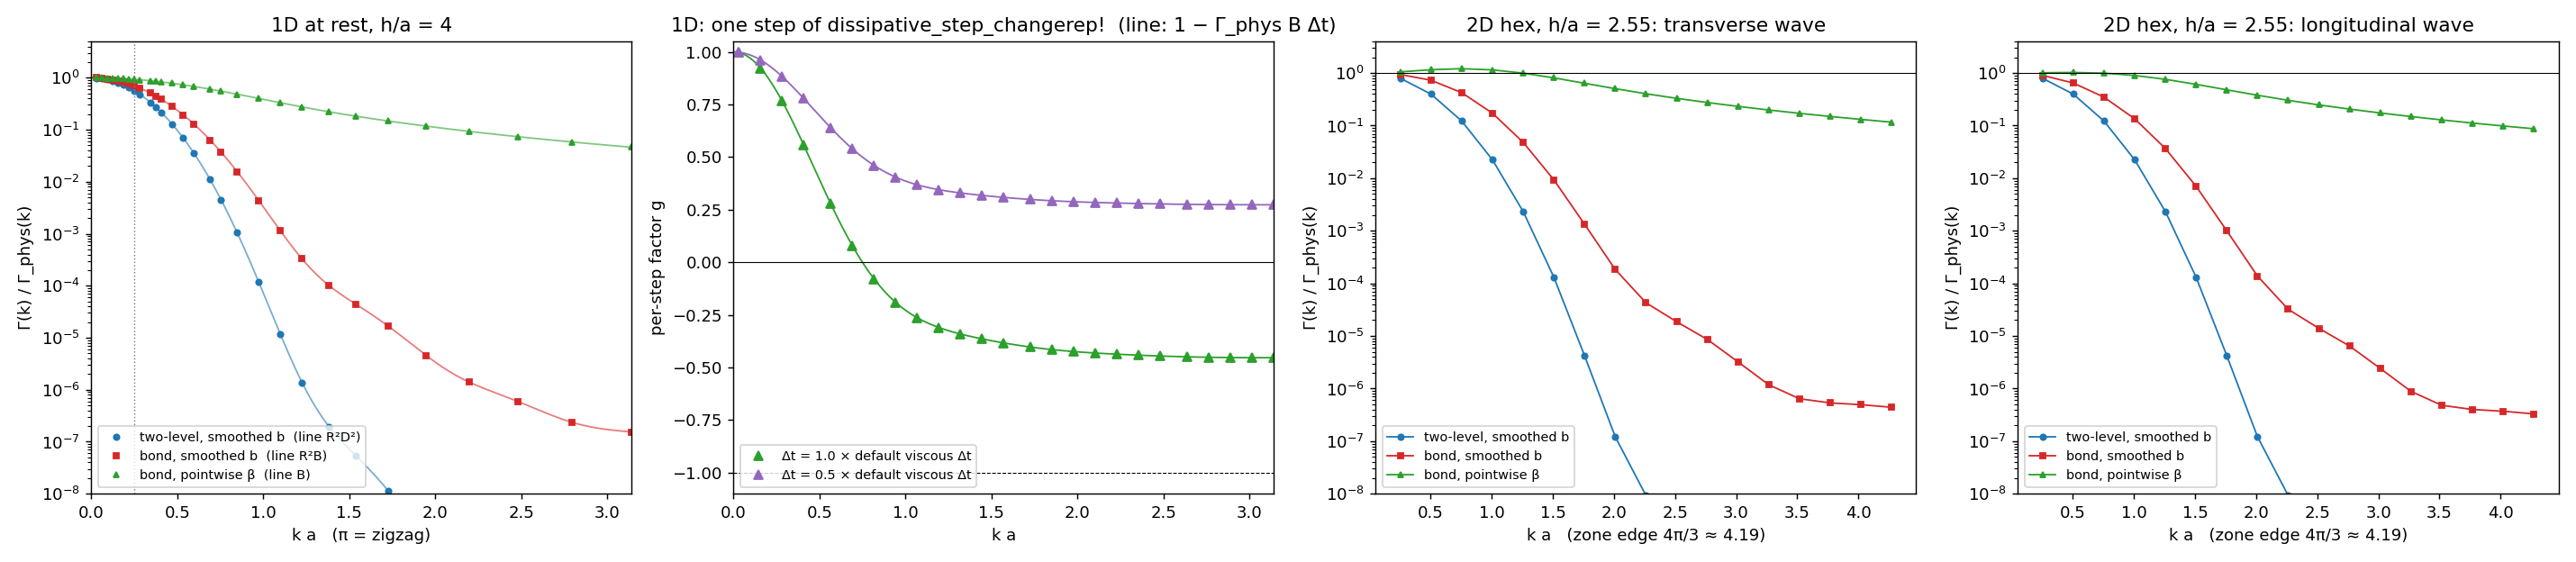
\includegraphics[width=\textwidth]{figs/changerep_damping.png}
\caption{Damping of a momentum wave on a frozen lattice at rest
(\texttt{examples/changerep\_damping.jl}).  First panel: 1D, $h/a=4$; points are
the code, lines the lattice formulas.  Second panel: the factor by which one
step of \texttt{dissipative\_step\_changerep!} multiplies the mode, at the default
viscous $\Delta t$ and at half of it.  Third and fourth panels: 2D hexagonal
lattice, $h/a=2.55$, transverse and longitudinal waves along $x$.}
\label{fig:damping}
\end{figure}

\paragraph{Rates.}  The measured rate is
$\Gamma=-\sum_a\bm F_a\cdot\bm m_a/\sum_a|\bm m_a|^2$ (\Fig{fig:damping}).
\begin{itemize}
\item \emph{1D.}  With the pointwise $\beta$ from the full EOS solve, the rate
  equals $B$ to $3\times10^{-11}$, over the whole zone.  With the smoothed
  $\beta$ it equals $R^2B$, to the $2\times10^{-4}$ of the discrete kernel
  normalization.  At the zigzag the pointwise rate is $0.046\,\Gamma_{\rm phys}$,
  against $1.5\times10^{-7}$ with $\beta$ and zero for the two-level form.
\item \emph{2D.}  The same holds for the mean-field bond form on the hexagonal
  lattice:
\end{itemize}
\begin{center}
\begin{tabular}{c c | c c c}
\hline\hline
$ka$ & & two-level, $\beta$ & bond, $\beta$ & bond, $\beta$\\
\hline
0.25 & T & 0.79 & 0.94 & 1.05\\
     & L & 0.79 & 0.90 & 1.01\\
1.51 & T & $1.3\times10^{-4}$ & $9.3\times10^{-3}$ & 0.81\\
     & L & $1.3\times10^{-4}$ & $7.0\times10^{-3}$ & 0.61\\
4.27 & T & $2\times10^{-14}$ & $4.4\times10^{-7}$ & 0.12\\
     & L & $2\times10^{-14}$ & $3.3\times10^{-7}$ & 0.087\\
\hline\hline
\end{tabular}
\end{center}
The pointwise rates tend to one at long wavelengths, overshoot mildly near
$ka\approx0.75$ (to $1.21$ for the transverse wave, where the resolved and
residual parts of the bond form are both sizable), and fall to about $0.1$ at
the zone edge.  So the change of representation removes the whole $R^2$ factor,
eight orders of magnitude at the zone edge.

\paragraph{The time step.}  One explicit step multiplies a mode by
\st
g=1-\Gamma\,\Delta t .
\stp
The measured $g$ agrees with this to $10^{-10}$, and the entropy produced equals
$2K\Delta t$ to $10^{-15}$.  But the larger rates matter for $\Delta t$.  The
default viscous step of \texttt{compute\_dt} is $\Delta t=0.2\,h^2w/\kappa$,
chosen when the short wavelengths were barely damped.  With the pointwise
$\beta$ the largest rate is $\Gamma_{\rm phys}B$ at the zone edge, and
\st
\max_k\Gamma\,\Delta t=1.45\qquad(\text{1D},\ h/a=4).
\stp
The step is still stable ($|g|<1$), but every mode with $\Gamma\Delta t>1$ changes
sign each step; at the zigzag $g=-0.45$.  Halving $\Delta t$ makes all factors
positive, with $g\ge0.27$.  The bound is set by the bond weight: the rate at
short wavelengths is about $(\kappa/w)\,2\mu_0/\mu_2$, with
$\mu_n=\sum_r\psi(r)|r|^n$, independent of $k$.  In 2D the full viscous $\Delta t$
exceeds $\Gamma\Delta t=2$ for the shortest modes, and the explicit step is
unstable.

\paragraph{The time-step criterion.}  The particle representation must
therefore take smaller time steps: its stronger damping of short wavelengths
sets $\Delta t$.  A bound on the fastest rate follows from Gershgorin's theorem
for the bond coefficients,
\st
\Gamma_{\max}\le4\,\frac{\kappa_b}{w}\,\max_a\sum_bw_{ab},\qquad
\sum_bw_{ab}\le d_s\frac{\int\psi}{\int\psi\,\rho^2}=\frac{c_d}{h_\psi^2},
\label{Gammabound}
\stp
with $c_1=15/4$ and $c_2=7/2$ for $\psi\propto(1-\rho/2h_\psi)^3$ (the continuum
integral includes $\rho\to0$, which the bond sum omits, so it bounds the lattice
sum), and $\kappa_b$ the largest viscosity the bonds carry: $\kappa(v=0)$ in 1D and
$2\eta+\zeta_{\rm eff}$ in 2D.  In 1D at $h/a=4$ the bound is $15\,\kappa/(wh^2)$,
twice the measured rate $7.3\,\kappa/(wh^2)$ of the zigzag mode.  For
\texttt{params.dissipation = :changerep}, \texttt{compute\_dt} requires
$\Gamma_{\max}\Delta t/2\le1$ for each viscous half step of \texttt{generic\_step!},
so the actual factor is at most about $1/2$ and every mode decays
monotonically.  This shortens the viscous time step to $0.67$ of the previous
value in 1D and $0.41$ in 2D ($h/a=2.5$).  \texttt{test/testchangerep.jl} checks it:
all per-step factors of the 1D lattice lie in $[0.52,1]$, and for a 2D random
field the kinetic energy decreases and the entropy increases at every half
step.

%=============================================================================
\section{Energy bookkeeping of the exact step}
\label{sec:energycheck}

\texttt{examples/changerep\_energy.jl} puts a momentum wave of wavenumber $k$ on
the 1D lattice of \Sect{sec:damping}, with velocity amplitude $10^{-2}$, and
applies the exact step at half the default viscous $\Delta t$ until the wave has
decayed by $10^{-4}$.  It records the kinetic energy
$\mathrm{KE}=\sum_a|\bm m_a|^2/(2wV_a)$ of the initial wave, the smoothed energy
$H$ before and after, the total particle energy, and the entropy produced:
\begin{center}
\begin{tabular}{c c | c c c | c c}
\hline\hline
$ka$ & $R_k^2$ & $(1-R_k^2)\,\mathrm{KE}$ & $\sum_ae_a-H_0$ & $H_{\rm end}-H_0$ &
drift of $\sum_ae_a$ & $T\,\Delta\mathbb S/\mathrm{KE}$\\
\hline
0.157 & 0.893 & $6.105\times10^{-6}$ & $6.118\times10^{-6}$ & $6.118\times10^{-6}$ & $10^{-11}$ & 1.0000\\
0.628 & 0.157 & $4.829\times10^{-5}$ & $4.829\times10^{-5}$ & $4.829\times10^{-5}$ & $2\times10^{-12}$ & 1.0000\\
1.257 & 0.001 & $5.720\times10^{-5}$ & $5.720\times10^{-5}$ & $5.720\times10^{-5}$ & $4\times10^{-11}$ & 1.0001\\
3.142 & 0     & $1.145\times10^{-4}$ & $1.145\times10^{-4}$ & $1.145\times10^{-4}$ & $8\times10^{-13}$ & 1.0001\\
\hline\hline
\end{tabular}
\end{center}
(At the zigzag $\cos^2kx_a=1$ on every particle, so its KE is twice that of the
other waves.)
\begin{itemize}
\item The excess $\sum_ae_a-H$ agrees with \Eq{excessk} to $2\times10^{-3}$, the
  size of the quartic terms at this amplitude.
\item $\sum_ae_a$ is conserved to round-off, as it must be: every $e_a$ is held
  fixed.
\item When the wave has decayed, $H$ has grown by exactly the initial excess,
  $H_{\rm end}=\sum_ae_a$.  The part $R_k^2\,\mathrm{KE}$ of the kinetic energy
  that $H$ already counted has turned into heat inside $H$; the part
  $(1-R_k^2)\,\mathrm{KE}$ that it did not count has been added to it.
\item All of the kinetic energy becomes heat, $T\,\Delta\mathbb S=\mathrm{KE}$.
\end{itemize}

\paragraph{Entropy per step.}  The exact entropy change of a step is smaller
than the first-order $2K\Delta t$ by the concave term of \Sect{sec:step}.  For a
mode damped at rate $\Gamma$, $\Delta\bm m=-\Gamma\Delta t\,\bm m$, and
\st
\Delta\mathbb S=2K\Delta t\,\Big(1-\frac{\Gamma\Delta t}{2}\Big),
\stp
which stays positive for every stable step, $\Gamma\Delta t<2$.  The measured
deficit in the first step is $2\%$ at $ka=0.16$ and $36\%$ at the zigzag, where
$\Gamma\Delta t=0.73$, as this formula predicts.  Over the whole decay the
deficits do not matter: the energy is exact, so the heat produced is exactly the
kinetic energy removed.

%=============================================================================
\section{Full deterministic runs}
\label{sec:hydro}

\texttt{examples/changerep\_hydro.jl} alternates viscous and Hamiltonian steps,
$D(\Delta t/2)\,H(\Delta t)\,D(\Delta t/2)$, on the 1D lattice ($h/a=4$), with the
viscous step $D$ done with the bond form on the smoothed $\beta$, as in
\texttt{generic\_step!}, or in the particle representation with the exact or the
gradient-corrected map of Appendix~\ref{sec:grad} (\Fig{fig:hydro}).  All runs here use the corrected
equation of state of Appendix~\ref{app:eos}.  Each half step uses $\Delta t/2$, so at the default viscous
$\Delta t$ every mode has $\Gamma\Delta t/2\le0.73$ and decays monotonically.

\begin{figure}[t]
\centering
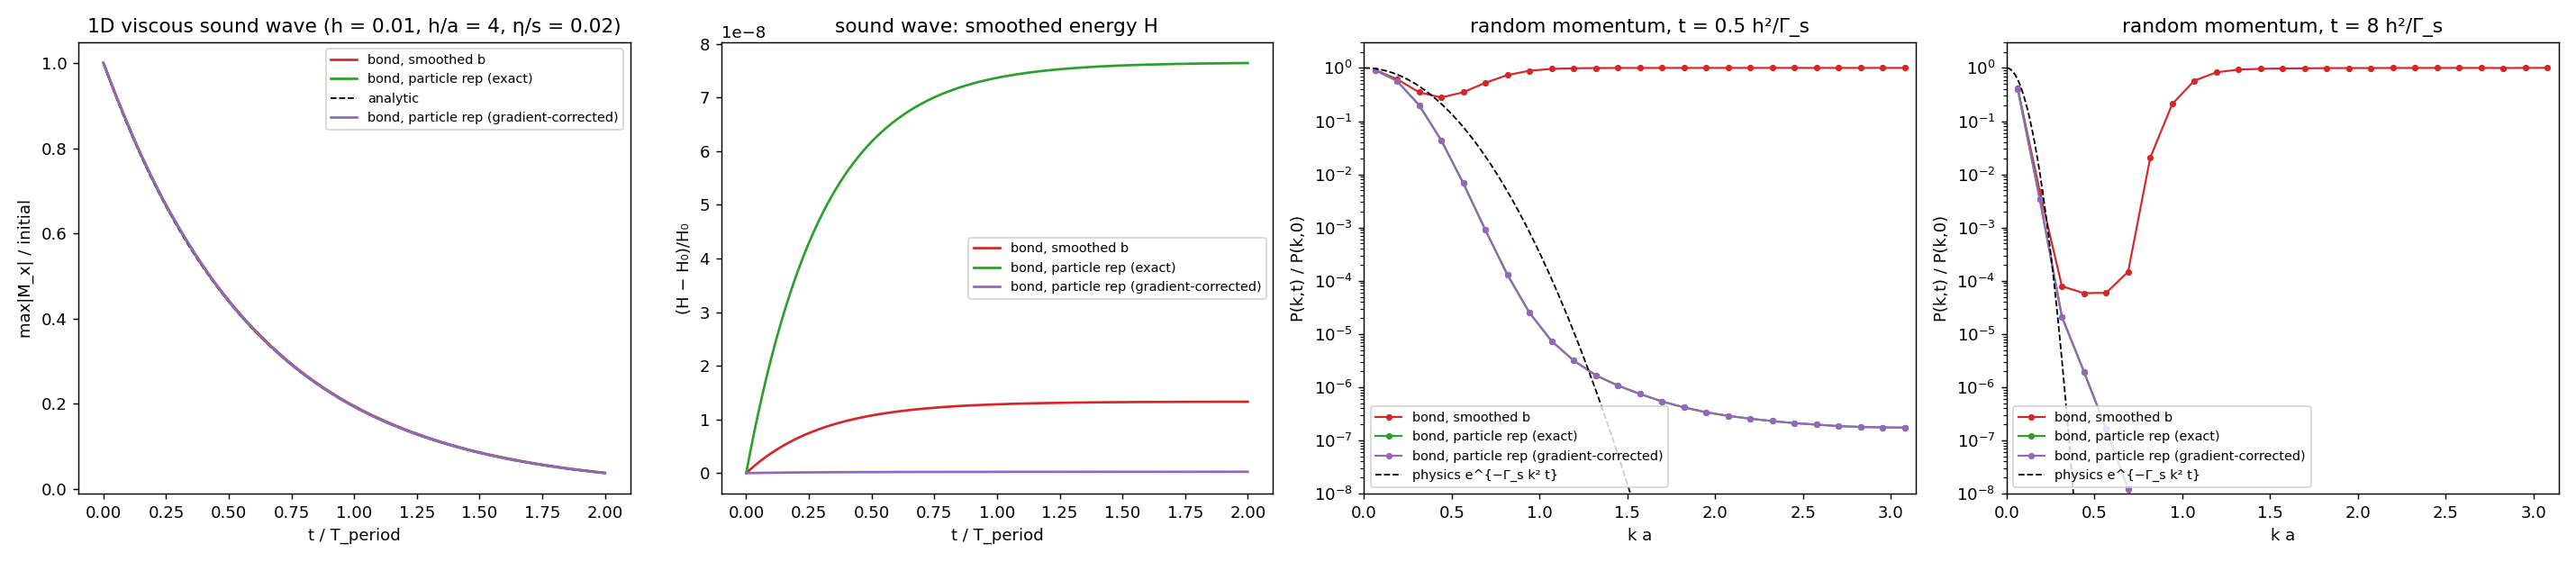
\includegraphics[width=\textwidth]{figs/changerep_hydro.png}
\caption{Full deterministic hydro in 1D (\texttt{examples/changerep\_hydro.jl}).
First two panels: a viscous sound wave ($h=0.01$, $\eta/s=0.02$, two periods),
amplitude and smoothed energy.  Last two panels: the spectrum of a random
momentum field ($h=0.02$, $\eta/s=0.1$) relative to its initial value, at
$t=0.5$ and $8$ in units of $h^2/\Gamma_s$, with $\Gamma_s=\kappa/w$.}
\label{fig:hydro}
\end{figure}

\paragraph{Viscous sound wave.}  The wave is resolved, $kh=0.13$.  After two
periods:
\begin{center}
\begin{tabular}{l c c c}
\hline\hline
 & smoothed $\beta$ & particle, exact & particle, gradient-corrected\\
\hline
amplitude (analytic $0.03713$) & $0.03775$ & $0.03719$ & $0.03719$\\
$\Delta S/S$ & $1.27\times10^{-5}$ & $1.27\times10^{-5}$ & $1.27\times10^{-5}$\\
$\Delta H/H$ & $1.3\times10^{-8}$ & $7.6\times10^{-8}$ & $2.5\times10^{-10}$\\
\hline\hline
\end{tabular}
\end{center}
Both particle versions follow the analytic decay more closely than the smoothed
$\beta$.  The exact map adds energy to $H$, the gradient part of the excess
released as the wave decays; the corrected map does not.

\paragraph{Random momentum field.}  Each particle starts with a random momentum
(velocity $\sim10^{-3}$) on a uniform fluid, so most of the kinetic energy is in
unresolved modes.
\begin{itemize}
\item With the smoothed $\beta$, the unresolved modes are not damped: for
  $ka\gtrsim1$ the spectrum stays at its initial value, and after $8h^2/\Gamma_s$
  $72\%$ of the kinetic energy is left.
\item In the particle representation every mode is damped.  After
  $8h^2/\Gamma_s$ only $1\%$ of the kinetic energy is left, and the resolved
  modes follow the physical decay.
\item At early times the intermediate modes, $0.5\lesssim ka\lesssim1.3$, decay
  faster than the physical sound damping $e^{-\Gamma_sk^2t}$.  Their pressure
  force passes through the smoothing, so they barely oscillate.  A propagating
  sound wave keeps half its energy as kinetic energy, which alone is damped; a
  mode that does not oscillate keeps all of it, so its momentum spectrum decays
  at twice the rate.
\end{itemize}
The energy bookkeeping is as in \Sect{sec:energycheck}:
\begin{center}
\begin{tabular}{l c c c}
\hline\hline
viscous step & $T\,\Delta S$ & $\Delta H$ & kinetic energy removed\\
\hline
smoothed $\beta$ & $1.14\times10^{-7}$ & $3.4\times10^{-9}$ & $3.2\times10^{-7}$\\
particle, exact & $1.12\times10^{-6}$ & $1.01\times10^{-6}$ & $1.12\times10^{-6}$\\
particle, gradient-corrected & $1.06\times10^{-6}$ & $0.95\times10^{-6}$ & $1.12\times10^{-6}$\\
\hline\hline
\end{tabular}
\end{center}
With the smoothed $\beta$ the scheme conserves $H$: the heat produced is kinetic
energy that $H$ already counted.  (The kinetic energy removed exceeds $T\Delta S$
there, because in the resolved modes, which oscillate, the Hamiltonian step also
turns kinetic energy into the energy of entropy fluctuations.)  In
the particle representation the heat produced is the kinetic energy removed,
and $H$ grows by the part of it that the smoothing did not count.  The gradient
correction leaves this almost unchanged: the energy of the random field is in the
residual, not in a smooth gradient, and it is still turned into heat.

%=============================================================================
\section{Two dimensions}
\label{sec:twod}

The same comparison in 2D, with the standard tests run unchanged and only the
viscous step replaced: the bond form on the smoothed $\beta$, as in
\texttt{generic\_step!}, or the step in the particle representation, with the exact
map or with the gradient-corrected map of Appendix~\ref{sec:grad}.  All runs use
the corrected equation of state of Appendix~\ref{app:eos}.

\paragraph{Viscous sound wave.}  \texttt{examples/changerep\_sound.jl} runs
\texttt{testsound\_viscous.jl} ($h=0.03$, $h/a=2$, $\eta/s=0.02$, one period;
\Fig{fig:sound2d}).  With the smoothed $\beta$ the wave is under-damped
throughout; in the particle representation the amplitude follows the analytic
decay closely:
\begin{center}
\begin{tabular}{l c c c}
\hline\hline
 & smoothed $\beta$ & particle, exact & particle, gradient-corrected\\
\hline
amplitude (analytic $0.2337$) & $0.2470$ & $0.2363$ & $0.2363$\\
$\Delta S/S$ & $1.172\times10^{-5}$ & $1.209\times10^{-5}$ & $1.172\times10^{-5}$\\
$\Delta H/H$ & $9.8\times10^{-8}$ & $5.1\times10^{-7}$ & $1.9\times10^{-8}$\\
\hline\hline
\end{tabular}
\end{center}
The gradient correction keeps the accuracy of the particle representation and
removes its energy gain; the entropy produced is then that of the smoothed
scheme.  On the final profile all runs share a small phase lead, which comes
from the smoothed sound speed rather than the viscous step.

\begin{figure}[t]
\centering
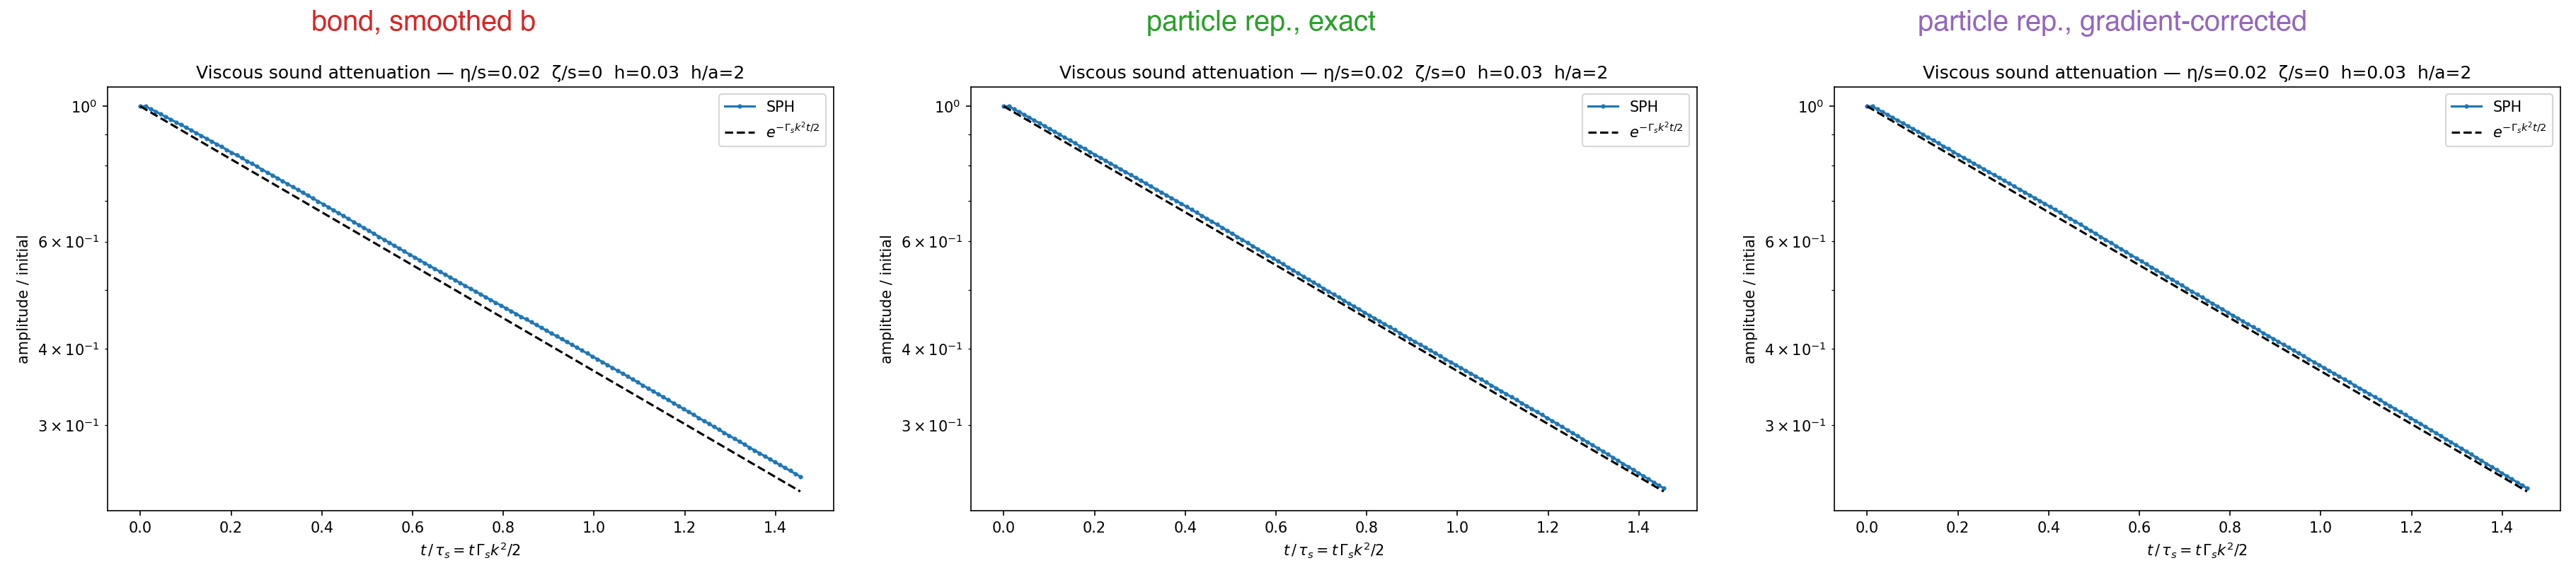
\includegraphics[width=\textwidth]{figs/changerep_sound2d_decay.png}\\[4pt]
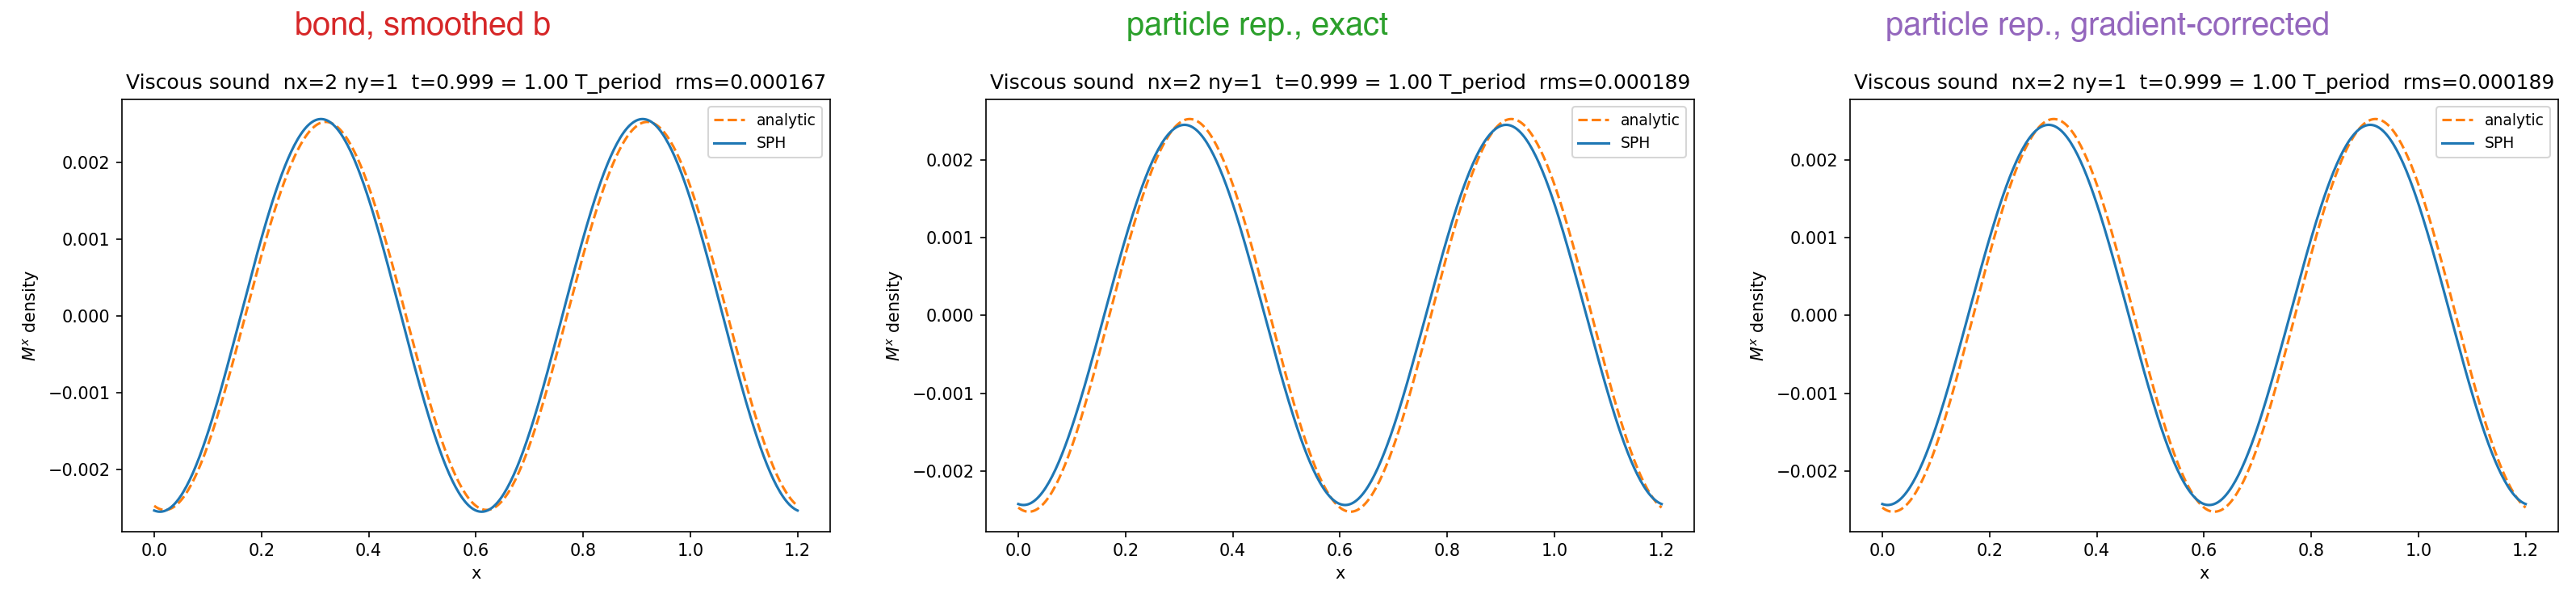
\includegraphics[width=\textwidth]{figs/changerep_sound2d_final.png}
\caption{2D viscous sound wave (\texttt{testsound\_viscous.jl}), with the viscous
step on the smoothed $\beta$ (left), in the particle representation with the
exact map (centre), and with the gradient-corrected map (right).  Top: amplitude
against $e^{-\Gamma_sk^2t/2}$.  Bottom: $M^x$ along $x$ after one period.}
\label{fig:sound2d}
\end{figure}

\paragraph{Gaussian.}  \texttt{examples/changerep\_gaussian\_lines.jl} evolves the
Gaussian of \texttt{testgaussian.jl} ($h=0.015$, $\eta/s=0.002$) with the smoothed
$\beta$ and with the gradient-corrected particle representation, and records
the energy density along the two axes through the centre at several times
(\Fig{fig:gaussian}).  The two schemes give the same flow at every time.  The
differences are at most $0.004$, against a peak of $1.1$, and have no systematic
sign; at $t=2.2$ they are below $0.0006$.  (With the exact map, the late-time
energy density was higher by about $0.002$ almost everywhere: the energy gain
discussed next, spread over the fluid as heat.)

\begin{figure}[t]
\centering
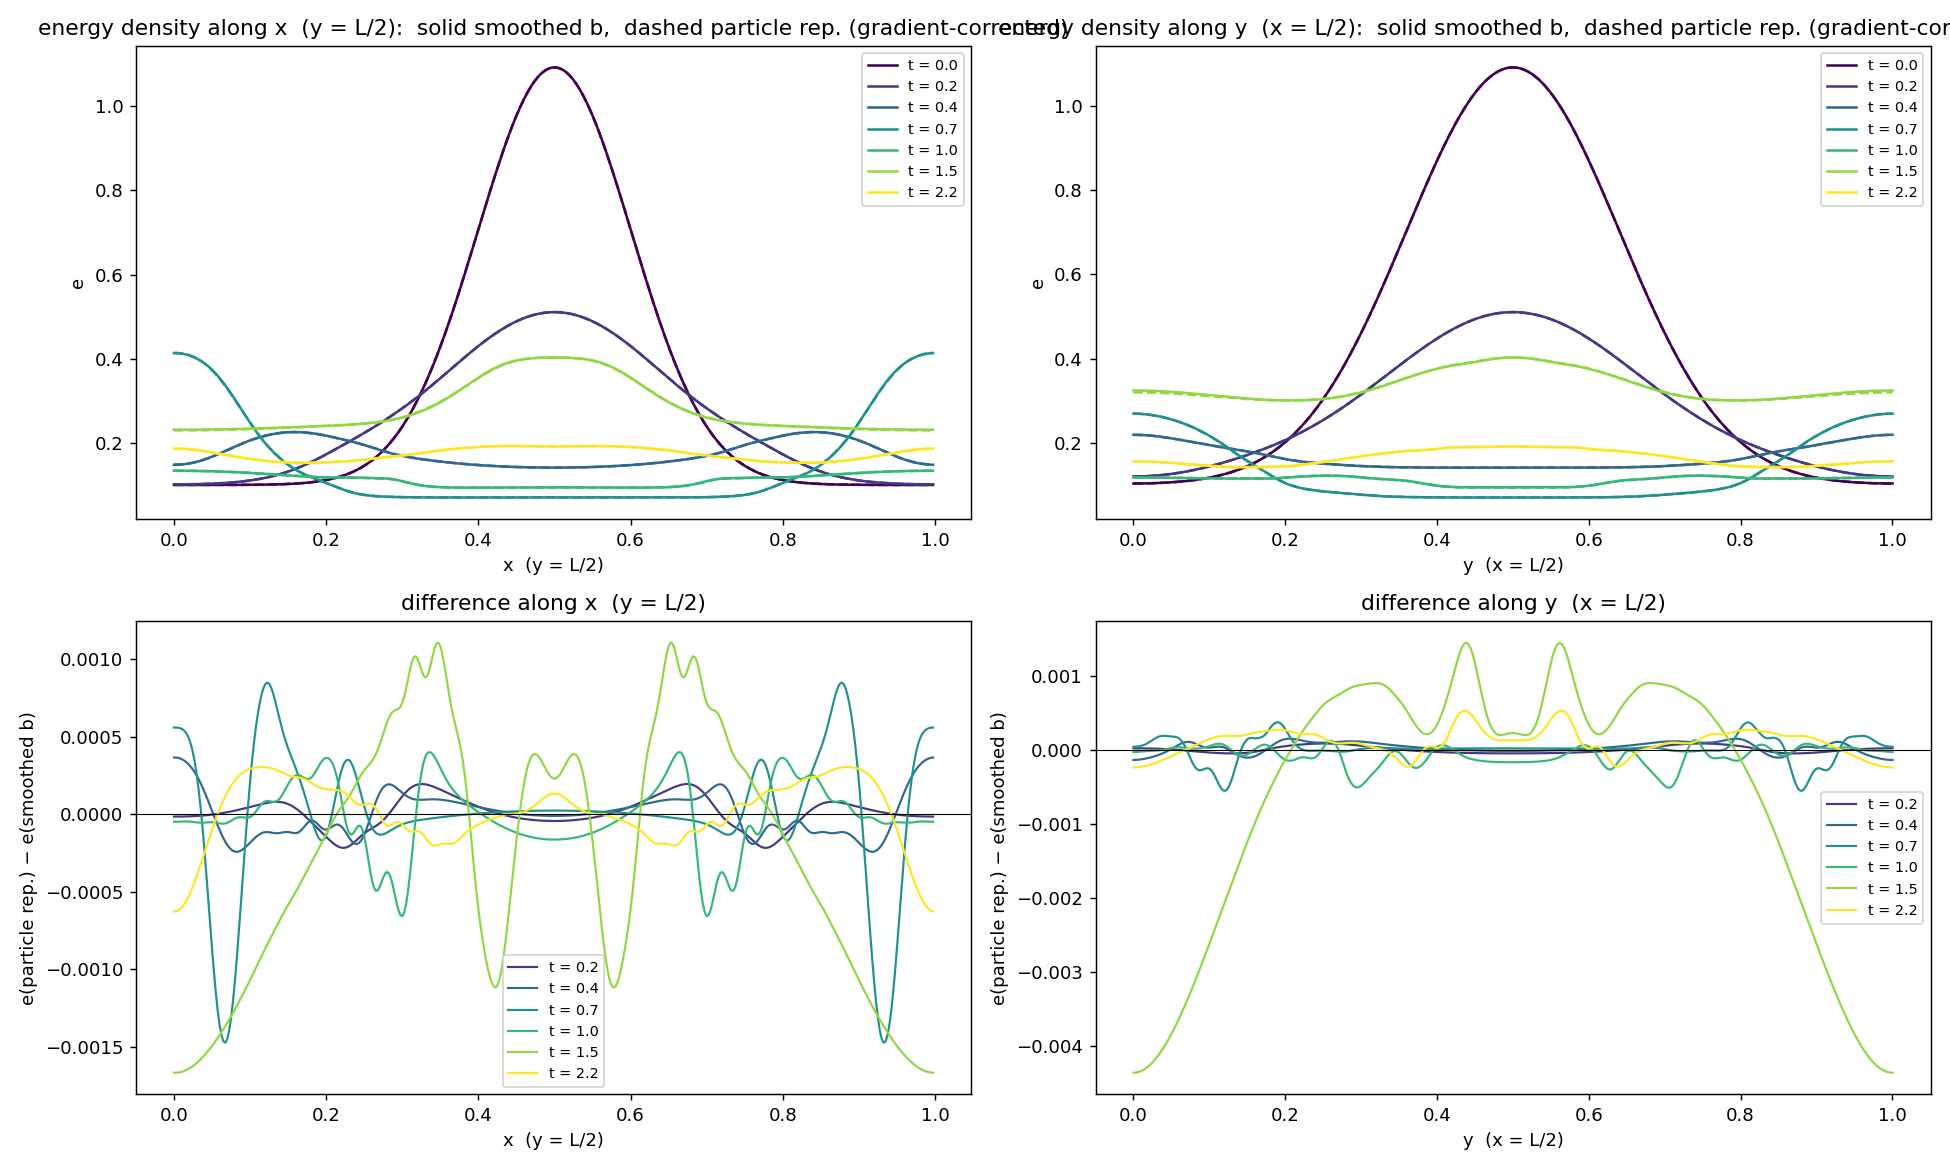
\includegraphics[width=\textwidth]{figs/changerep_gaussian_lines.png}
\caption{2D Gaussian: energy density along $x$ (left) and $y$ (right) through
the centre, at $t=0$ to $2.2$.  Top: smoothed $\beta$ (solid) and particle
representation with the gradient-corrected map (dashed).  Bottom: their
difference.}
\label{fig:gaussian}
\end{figure}

\paragraph{Long-time energy.}  The leapfrog conserves a nearby (shadow)
Hamiltonian, not $H$ itself, so $H$ oscillates; what matters is whether it
drifts.  For resolved viscous hydro every scheme should give, as $h\to0$, a
constant $H(t)$ and the same growing $S(t)$.
\texttt{examples/changerep\_energy\_drift.jl} records $H(t)$ and $S(t)$ after every
full step for the Gaussian at $h=0.03$ up to $t=4$ (\Fig{fig:drift}):
\begin{itemize}
\item The two-level form and the bond form on the smoothed $\beta$ give the same
  $H(t)$, constant to $3\times10^{-4}$.
\item With the exact map, $H$ grows steadily, to $2.7\times10^{-3}$ at $t=4$, and
  the entropy grows faster.
\item With the gradient-corrected map, $H(t)$ and $S(t)$ follow the smoothed
  schemes.
\end{itemize}

\begin{figure}[t]
\centering
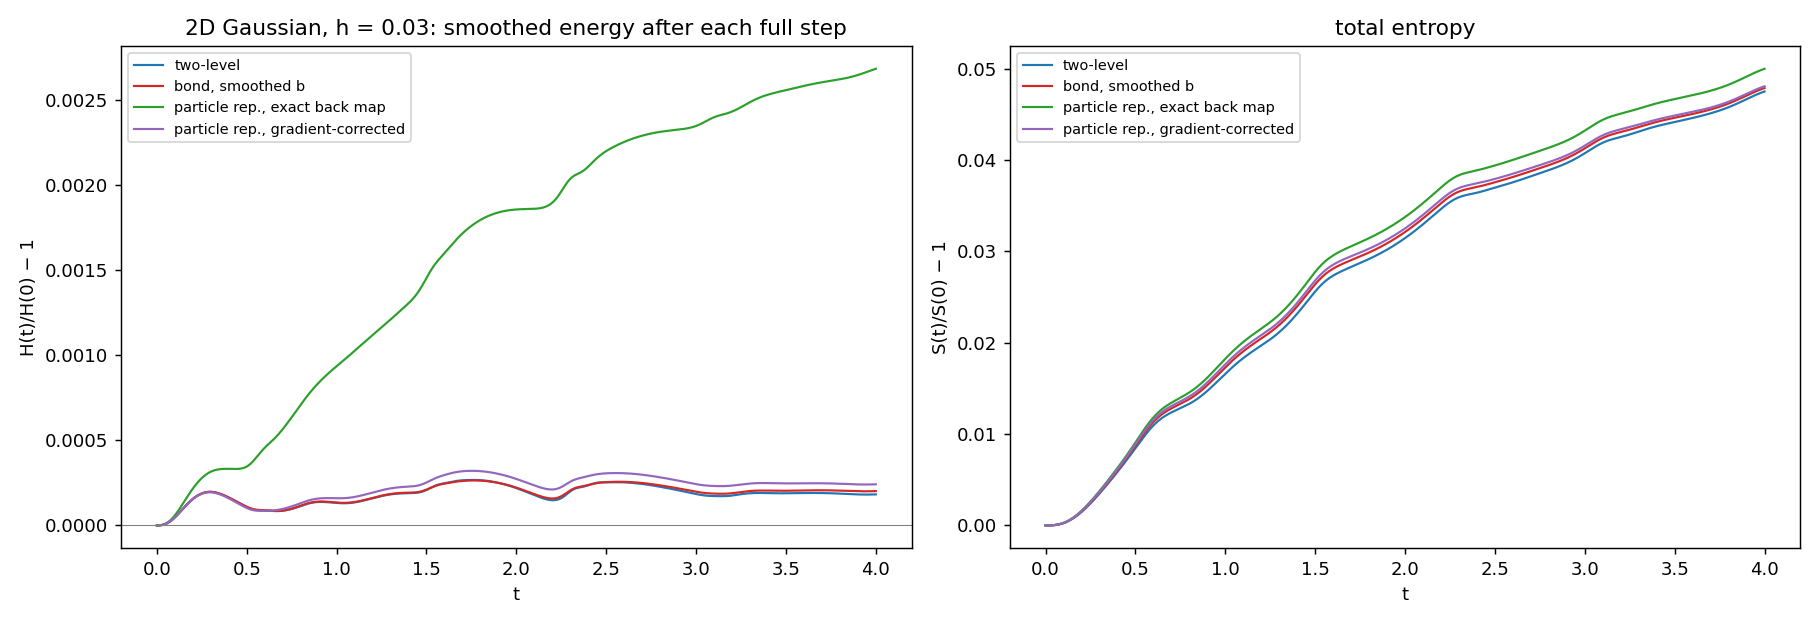
\includegraphics[width=\textwidth]{figs/changerep_energy_drift.png}
\caption{2D Gaussian at $h=0.03$: smoothed energy (left) and total entropy (right)
after each full step.}
\label{fig:drift}
\end{figure}

\paragraph{Convergence.}  \texttt{examples/changerep\_convergence.jl} repeats this
at $h=0.045$, $0.03$, $0.0225$ and $0.015$ up to $t=3$
(\Fig{fig:convh}, and \Fig{fig:conv} in the appendix).
\begin{itemize}
\item \emph{The particle representation works without any correction, provided
  $h$ is small enough.}  With the exact map the late-time energy gain is
  $4.9$, $2.3$, $1.3$ and $0.58\times10^{-3}$: it converges as $h^2$.  The entropy
  produced converges to that of the smoothed schemes, $4.27\%$ against
  $4.20$--$4.22\%$ at $h=0.015$.
\item The gain is secular: the excess energy is proportional to the entropy
  produced, $\Delta H_{\rm excess}/H\simeq c\,h^2\,\Delta S/S$ with
  $c/h^2\approx60$ (third panel of \Fig{fig:convh}).  Every unit of viscous heat
  comes with an extra energy of relative size $\propto h^2$: the smooth-gradient
  part of the excess, released along with the physical dissipation.
\item The gradient-corrected map removes the lion's share of this secular gain:
  the excess per entropy produced drops by a factor $10$ at $h=0.045$, $30$ at
  $h=0.03$, and to the level of the smoothed schemes at smaller $h$.
\end{itemize}

\begin{figure}[t]
\centering
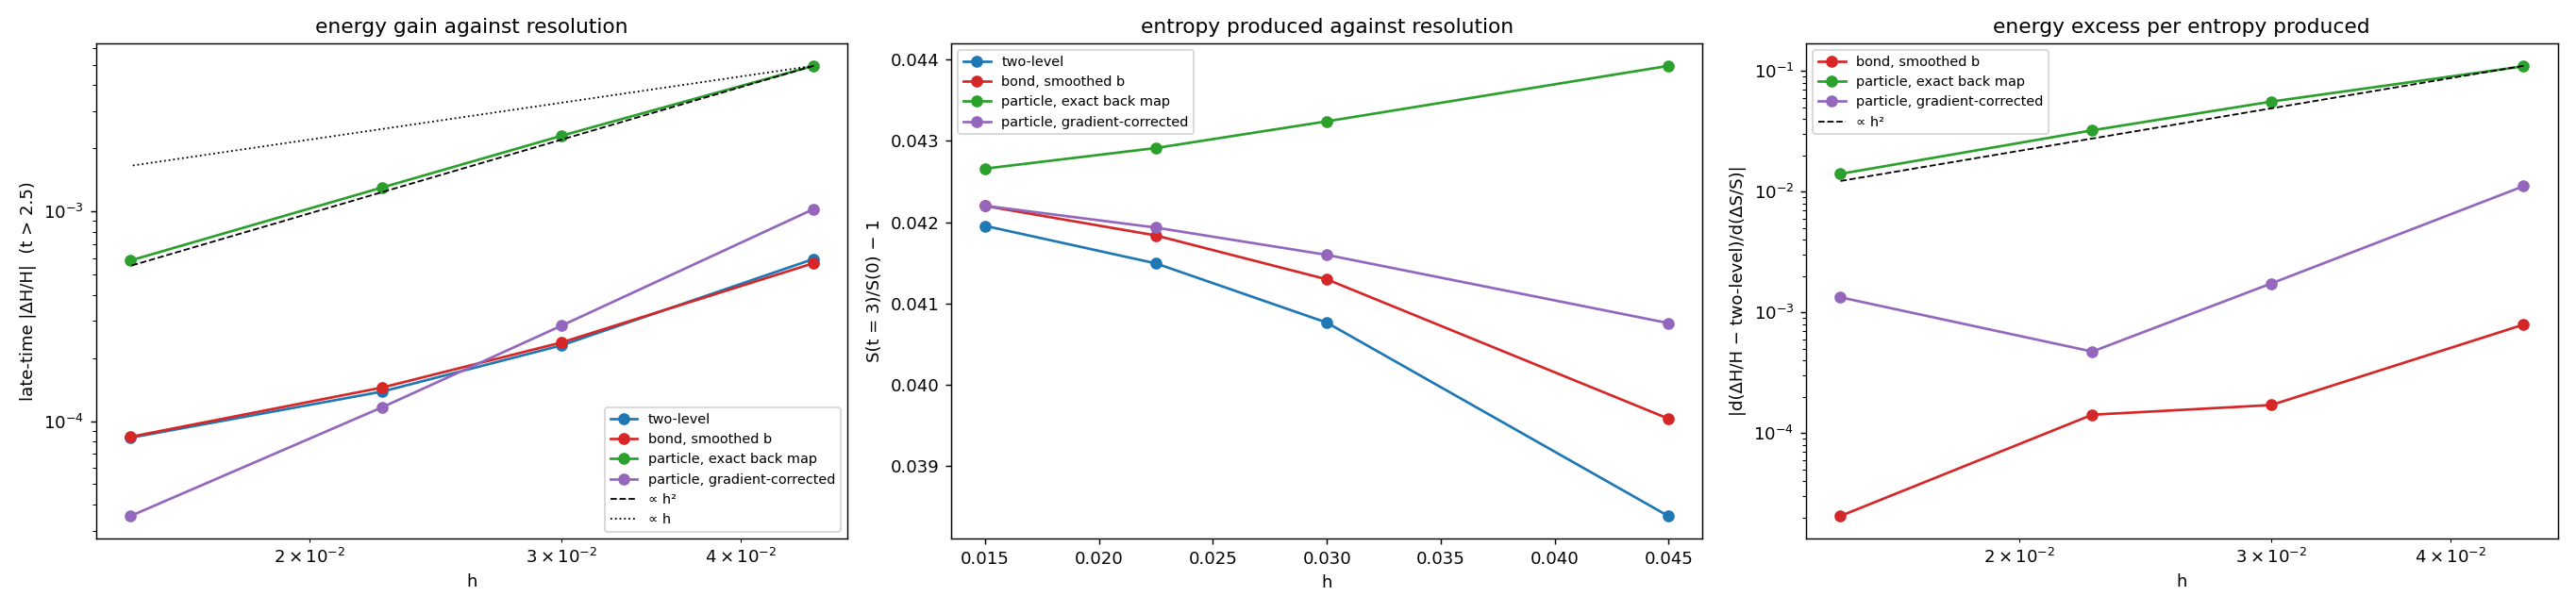
\includegraphics[width=\textwidth]{figs/changerep_convergence_h.png}
\caption{2D Gaussian, convergence in $h$.  Left: late-time energy gain
($t>2.5$).  Centre: entropy produced at $t=3$.  Right: slope of the energy excess
over the two-level form against the entropy produced.}
\label{fig:convh}
\end{figure}

%=============================================================================
\section{Open points}
\label{sec:open}

The gradient-corrected particle representation is now the default viscous step
of the code, \texttt{params.dissipation = :changerep}; \texttt{test/testchangerep.jl}
checks the conversion map, the rates of \Sect{sec:damping}, the gradient
correction and conservation.

\begin{itemize}
\item \emph{Speed.}  The gradient-corrected step is several times slower than the
  bond step on the smoothed $\beta$: each half step rebuilds every particle's
  kernel star and fits $G_a$ twice, with a pseudo-inverse.  Closed-form $2\times2$
  fits, reused neighbour lists and a single pass over the stars should bring it
  close to the cost of the bond step.
\item \emph{The force of the corrected map.}  The gradient correction adds a
  higher-derivative term to the thermodynamic force,
  \Eq{betaeff}; it is not yet included in the force.
\item \emph{Time step.}  An implicit or exponential update of the bond step
  would remove the time-step restriction of \Sect{sec:damping}, which the code now
  enforces (below).
\item \emph{Stochastic step.}  Random momentum transfers between pairs,
  accepted with the exact $\Delta\mathbb S$; their mean drift should reproduce
  the deterministic rates of \Sect{sec:damping}.
\end{itemize}

%=============================================================================
\appendix
\section{A gradient-corrected conversion map}
\label{sec:grad}

\paragraph{The smooth part of the excess.}  By \Eq{excess}, the particle energies
exceed $H$ by the local variance of $\bm\mu$ around each particle.  For a smooth
flow the deviations are not fluctuations but the gradient across the star.  With
$\bar{\bm r}_a=\sum_b\lambda_{ab}\bm r_{ab}$ the centre of the star (zero on a
symmetric one),
\st
\delta\bm\mu_{ab}\simeq\nabla\bm\mu\cdot\big(\bm r_{ab}-\bar{\bm r}_a\big),
\stp
and the excess contains
\st
g_a=\frac12\,s_a\,(G_a)_{ij}\,C_a^{ik}\,(G_a)_{kl}\,Q_a^{jl},\qquad
Q_a^{jl}=\sum_b\lambda_{ab}\,(r_{ab}-\bar r_a)^j(r_{ab}-\bar r_a)^l ,
\label{ga}
\stp
with $G_a$ the gradient of $\bm\mu$ at $a$.  $Q_a$ is the second moment of the
kernel, of order $h^2$, so even a perfectly resolved flow has an excess of order
$h^2|\nabla\bm\mu|^2$ per unit entropy.  The uncorrected step holds every $e_a$
fixed, so as viscosity reduces the gradient it adds $\sum_a\Delta g_a$ to $H$.
That is energy the smoothed representation already counted, as part of the
resolved flow; ordinary viscosity would leave $H$ unchanged.

\paragraph{The corrected map.}  Treat the linear part of the variation as
resolved, and only the residual as the particle's own fluctuation.  Take $G_a$
to be the least-squares gradient of $\bm\mu$ on the star of $a$ with the kernel
weights $\lambda_{ab}$ (the construction of \texttt{bond\_dissipation.tex}, with
these weights in place of the bond weights), so that the residual
\st
\delta\bm\mu'_{ab}=\bm\mu_b-\bar{\bm\mu}_a-G_a\big(\bm r_{ab}-\bar{\bm r}_a\big)
\stp
is orthogonal to the linear part, $\sum_b\lambda_{ab}\,\delta\bm\mu'_{ab}(\bm r_{ab}-\bar{\bm r}_a)^T=0$.
The cross term in the variance then vanishes for any $C_a$, and the excess
splits exactly, at quadratic order, into $\sum_ag_a$ and the variance of the
residual.  The step becomes:
\begin{enumerate}
\item \emph{Forward:} $e_a'=e_a-g_a$, with $e_a$ the energy the equation of state
  assigns to $(s_a,\bm m_a)$ at volume $V_a$.
\item \emph{Transfer:} move momentum between particles at fixed $e_a'$.
\item \emph{Back:} recompute the fit $G_a'$ from the new momenta, hence $g_a'$, and
  set
  \st
  s_a'=S_a\big(e_a'+g_a',\ \bm m_a'\big).
  \stp
\end{enumerate}
The gradient energy moves with the resolved flow, as $H$ treats it, and only the
variance of the residual is turned into heat.  For a resolved flow the step
then conserves $H$, like ordinary viscosity, while the particle-scale
fluctuations are still released.  It is the resolved-plus-residual split of the
bond form, applied to the conversion map.

\paragraph{Maximizing entropy at fixed constraints.}  Both versions of the step
increase the total particle entropy at fixed constraints.
\begin{itemize}
\item \emph{Uncorrected.}  Every $e_a$ is held fixed, and the step increases
  \st
  \mathbb S=\sum_aS_a(e_a,\bm m_a)
  \stp
  over the momenta, at fixed total momentum.  The constraints are local, and
  the force conjugate to $\bm m_a$ is $\beta_a=-\partial S_a/\partial\bm m_a$.
\item \emph{Corrected.}  The constraint becomes
  \st
  e_a'=e_a-g_a[\bm m]=\text{const},
  \stp
  and $g_a$ depends on the neighbours' momenta through the fitted gradient
  $G_a$.  The constraint now contains a square-gradient term, with a coefficient
  set by the kernel's second moment, of order $h^2$.  Equivalently the step
  increases
  \st
  \mathbb S'=\sum_aS_a\big(e_a'+g_a[\bm m],\ \bm m_a\big)\qquad\text{at fixed }e_a' .
  \stp
\end{itemize}
Differentiating with respect to $\bm m_c$, the derivative term adds to the
thermodynamic force
\st
\beta_c^{\rm eff}=\beta_c-\sum_a\frac1{T_a}\,\frac{\partial g_a}{\partial\bm m_c} .
\label{betaeff}
\stp
Since $g_a$ is quadratic in the gradient, the correction is a discrete
divergence of $C\,\nabla\bm\mu$: a higher-derivative correction of order $h^2$.
Summed over particles, the corrected constraint is
\st
\sum_ae_a'=\sum_ae_a-\sum_ag_a\simeq H+(\text{variance of the residual}),
\stp
so the derivative term moves the constraint from $\sum_ae_a$ towards the resolved
energy $H$ plus the energy of the particle-scale fluctuations.

\paragraph{Implementation.}  \texttt{dissipative\_step\_changerep\_grad!} in
\texttt{src/changerep.jl}:
\begin{enumerate}
\item smooth, and for each particle build its star with the kernel weights
  $\lambda_{ab}$, the centred second moment $Q_a$, the fitted gradient $G_a$ of
  $\bm\mu$, and $C_a$ of \Eq{Canalytic} at the smoothed state;
\item set $e_a'=e_a-g_a$;
\item compute the particle forces $\beta_a$, the bond force, and
  $\Delta\bm m_a=\Delta t\,\bm F_a$;
\item refit $G_a'$ from the new momenta on the same stars, and set
  $s_a'=S_a(e_a'+g_a',\bm m_a')$.
\end{enumerate}
The force uses the uncorrected $\beta_a$; the derivative term of $\beta^{\rm eff}$
is not included.

\paragraph{The inverse susceptibility.}  $C_a=\partial^2f_a/\partial\bm\mu\,\partial\bm\mu
=S\,\partial\bm v/\partial\bm M|_S$ has a closed form.  At fixed $S=s\gamma$ the
entropy per volume changes as $ds/s=-d\gamma/\gamma$, so with $ds/de=s/w$ the
rest-frame energy density changes as $de=-w\,d\ln\gamma$, and $dw=(1+c_s^2)\,de$.
Differentiating $\bm M=w\gamma^2\bm v$, with $d\gamma=\gamma^3\,\bm v\cdot d\bm v$,
\st
\frac{\partial\bm M}{\partial\bm v}\Big|_S=w\gamma^2\big[\one+\gamma^2(1-c_s^2)\,\bm v\bm v^T\big],
\stp
and inverting,
\st
C=S\,\frac{\partial\bm v}{\partial\bm M}\Big|_S
=\frac{1}{T\gamma^2}\left[\one-\frac{(1-c_s^2)\,\bm v\bm v^T}{1-c_s^2v^2}\right],
\qquad T=\frac{e+p}{S}=\frac{T_{\rm rel}}{\gamma} .
\label{Canalytic}
\stp
Transverse to $\bm v$ it is $1/(T\gamma^2)$, along $\bm v$ it is
$1/[T\gamma^4(1-c_s^2v^2)]$, and at rest it is $\one/T$.  It agrees with a
finite-difference evaluation through the equation of state to $10^{-10}$ up to
$v=0.83$.

\paragraph{A first check.}  For a smooth shear flow on the 2D lattice
($\bm\mu\propto\sin2\pi x\,\hat y$, $h=0.05$), the gradient energy $\sum_ag_a$
accounts for $98.8\%$ of the excess $\sum_ae_a-H$.  In one viscous step, the
change of $H$ relative to the heat produced, $\Delta H/(T\Delta S)$, is $0.027$ for
the uncorrected exact step and $0.0004$ for the corrected one.

\paragraph{Convergence.}  \Fig{fig:conv} shows $H(t)$ and $S(t)$ for the
Gaussian at four resolutions, for the two smoothed schemes and the two maps of
the particle representation.  The late-time energy gain, $\Delta H/H$ for $t>2.5$:
\begin{center}
\begin{tabular}{c | c c c c}
\hline\hline
$h$ & two-level & bond, smoothed $\beta$ & particle, exact & particle, gradient-corrected\\
\hline
0.045  & $5.9\times10^{-4}$ & $5.7\times10^{-4}$ & $4.9\times10^{-3}$ & $1.0\times10^{-3}$\\
0.03   & $2.3\times10^{-4}$ & $2.4\times10^{-4}$ & $2.3\times10^{-3}$ & $2.9\times10^{-4}$\\
0.0225 & $1.4\times10^{-4}$ & $1.4\times10^{-4}$ & $1.3\times10^{-3}$ & $1.2\times10^{-4}$\\
0.015  & $8.3\times10^{-5}$ & $8.4\times10^{-5}$ & $5.8\times10^{-4}$ & $3.5\times10^{-5}$\\
\hline\hline
\end{tabular}
\end{center}
With the gradient correction, the energy gain is that of the smoothed schemes,
or smaller at fine resolution, and the entropy produced agrees with the bond form
on the smoothed $\beta$: $4.220\%$ against $4.220\%$ at $h=0.015$.  The slope of the
excess energy against the entropy produced (\Fig{fig:convh}) is
$1.1\times10^{-2}$, $1.7\times10^{-3}$, $-0.5\times10^{-3}$ and $-1.3\times10^{-3}$,
against $0.109$, $0.056$, $0.032$ and $0.014$ for the exact map.  The correction is
not exact---the force still uses the uncorrected $\beta_a$, and $g_a$ captures the
smooth excess only to quadratic order---but it removes most of the secular gain.

\begin{figure}[t]
\centering
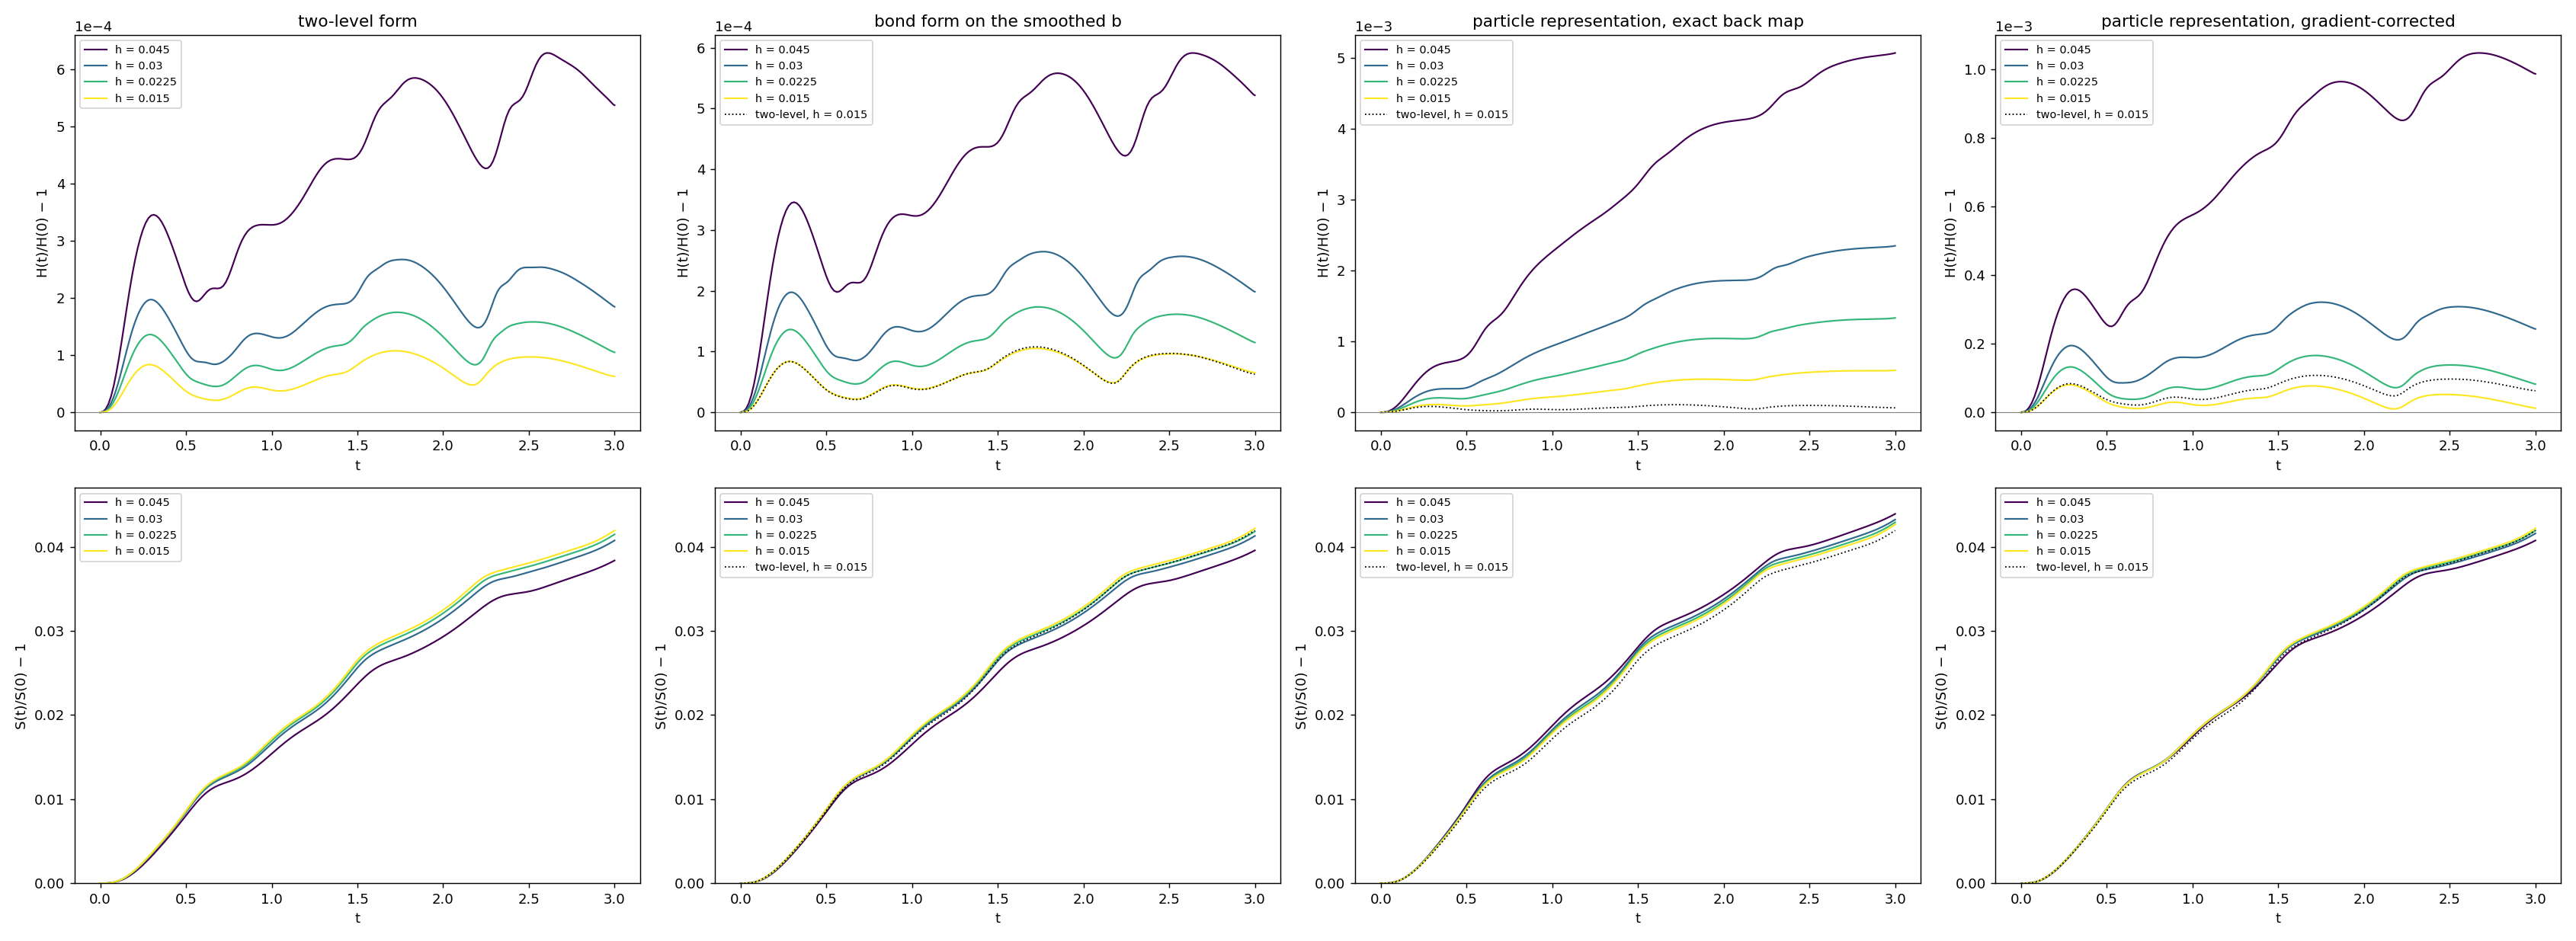
\includegraphics[width=\textwidth]{figs/changerep_convergence.png}
\caption{2D Gaussian, $H(t)$ (top) and $S(t)$ (bottom) at $h=0.045$ to $0.015$ for
the two-level form, the bond form on the smoothed $\beta$, and the particle
representation with the exact and the gradient-corrected map.  Each panel has
its own vertical scale.  Dotted: two-level at $h=0.015$.}
\label{fig:conv}
\end{figure}


%=============================================================================
\section{The equation-of-state inversion}
\label{app:eos}

The energy studies of this note exposed an error in \texttt{solve\_eos!}, which
was corrected before the runs reported here (\texttt{test/testeos\_consistency.jl}).

\paragraph{The error.}  The Hamiltonian uses the energy density
$h=(e+p)\gamma^2-p$ as a function of the entropy density $S=s\gamma$ and the
momentum density.  This energy is conjugate to the density-frame momentum
\st
M^i=(e+p)\gamma^2v^i=(e+p)\gamma\,u^i ,
\stp
for which $\partial h/\partial\bm M=\bm v$ and $\partial h/\partial S=(e+p)/S$, and
for which the post-convergence expression for $\mathcal F/S$ follows from the
Euler relation $h+p=TS+\bm v\cdot\bm M$.  The solver instead took
$\bm u=\bm M/(e+p)$, dropping a factor $\gamma$ (the same step was missing in
\texttt{sph2.tex}, \S II.4).  For a moving fluid the energy was then not conjugate
to the momentum: the Hamiltonian velocity $\dot{\bm x}_a$ and $T_{\rm eff}$ were not
the derivatives of $H$, wrong at $O(v^2)$ (by $10$--$20\%$ at $v\approx0.2$--$0.35$).

\paragraph{Consequences.}  Neither the leapfrog nor any viscous step could
conserve $H$ in a moving flow; even the two-level step changed $H$ at first order
in $\Delta t$.  The resolved, slow flows of the standard tests were hardly
affected, since the error is $O(v^2)$.  The energy studies of this note were the
first to require exact bookkeeping in a strongly moving flow.  With the corrected
solver the oscillation of $H$ in the Gaussian drops from $8\times10^{-3}$ to
$3\times10^{-4}$, the exact and first-order entropy updates of the particle
representation agree, and the energy gain converges as $h^2$.


\end{document}
